\documentclass[polish]{beamer}

% wide screen
% \documentclass[aspectratio=169]{beamer}


%%% YOUR PACKAGES HERE %%%
\usepackage{comment}
\usepackage{hyperref}
\usepackage{tikz} 
\usetikzlibrary{graphs,graphs.standard,automata}


% polish language
\usepackage[polish]{babel}
\usepackage{polski}



%%% IMPORT PG PRESENTATION STYLE %%%
% THIS IS GDANSK UNIVERSITY OF TECHNLOGOGY (PG) PRESENTATION TEMPLATE
% Creator: Jan Cychnerski <jan.cychnerski@eti.pg.edu.pl>
% Copyleft 2019


% PG THEME OPTIONS

\usetheme{Boadilla}
\usecolortheme{default}
\usefonttheme{professionalfonts}

% colors

\definecolor{PGBlue}{RGB}{0,56,101}
\definecolor{PGRed}{RGB}{193,10,39}
\definecolor{PGSilver}{RGB}{200,200,200}
\definecolor{PGBlack}{RGB}{0,0,0}

% PGBlue
\setbeamercolor{frametitle}{fg=PGBlue}
\setbeamercolor{normal text}{fg=PGBlue}
\setbeamercolor{structure}{fg=PGBlue}
\setbeamercolor{item}{fg=PGBlue}

% PGRed
\setbeamercolor{alerted text}{fg=PGRed}
\setbeamercolor{item projected}{fg=PGRed}

% white
\setbeamercolor{title}{fg=white}
\setbeamercolor{titlelike}{fg=white}
\setbeamercolor{subtitle}{fg=white}

% enumerate and itemize styles

\setbeamertemplate{itemize item}{\bfseries\color{PGRed}\raise1pt\hbox{\donotcoloroutermaths$\bullet$}}
\setbeamertemplate{itemize subitem}{\color{PGRed}\raise0.5pt\hbox{--}}
\setbeamertemplate{itemize subsubitem}{\color{PGRed}\tiny\raise1.5pt\hbox{\donotcoloroutermaths$\bullet$}}

\setbeamertemplate{enumerate item}{\bfseries\color{PGRed}\insertenumlabel.}
\setbeamertemplate{enumerate subitem}{\color{PGRed}\insertsubenumlabel.}
\setbeamertemplate{enumerate subsubitem}{\color{PGRed}\insertsubsubenumlabel.}
\setbeamertemplate{enumerate mini template}{\insertenumlabel}


% disable navigation

\beamertemplatenavigationsymbolsempty

% additional commands

\newcommand*{\vcenteredhbox}[1]{\begingroup
\setbox0=\hbox{#1}\parbox{\wd0}{\box0}\endgroup}

\graphicspath{{pgbeamer/}}


\usepackage{iflang}
\IfLanguageName{polish}{
\newcommand{\pglogobig}{pg-logo-big-pl}
\newcommand{\pglogosmall}{pg-logo-small-pl}
}{
\newcommand{\pglogobig}{pg-logo-big-en}
\newcommand{\pglogosmall}{pg-logo-small-en}
}


% FRAME TITLE LOGO
\addtobeamertemplate{frametitle}{\vcenteredhbox{\includegraphics[height=8mm]{\pglogosmall}}\bfseries}{}


\newcommand{\pgtitleframe}{{
% PG TITLE PAGE

\setbeamercolor{background canvas}{bg=PGBlue}
\setbeamercolor{title}{fg=white}
\setbeamercolor*{date}{fg=white}
\setbeamercolor*{author}{fg=white}

\setbeamertemplate{footline}{}

\begin{frame}[noframenumbering]
\centering
\vspace{1cm}
\includegraphics[height=3cm]{\pglogobig}
\vspace{5mm}
\maketitle
\end{frame}
}}

\newcommand{\pglastframe}{{
% PG LAST PAGE

\setbeamercolor{background canvas}{bg=PGBlue}
\setbeamercolor{title}{fg=white}
\setbeamercolor*{date}{fg=white}
\setbeamercolor*{author}{fg=white}

\setbeamertemplate{footline}{}

\begin{frame}[noframenumbering]
\centering
\vspace{1cm}
\includegraphics[height=5cm]{\pglogobig}
\end{frame}
}}



%%% YOUR OPTIONS HERE %%%

\title[Eternally surrounding a robber]{Eternally surrounding a robber}
\subtitle{czyli jak sprawić, aby nie było dojścia do prezydenta.}
\author{Marek Borzyszkowski}
\date{\today}

\setbeamercovered{transparent}



%%% DOCUMENT BEGINS HERE %%%

\begin{document}

\tikzset{vertex/.style={circle, draw=black, radius=1cm}}
\tikzset{cop_vertex/.style={vertex, fill=blue!50}}
\tikzset{rob_vertex/.style={vertex, fill=red!50}}
\tikzset{cop_rob_vertex/.style={vertex, fill=green!50}}
\tikzset{edge/.style={black}}

%%% PG TITLE PAGE %%%
\pgtitleframe

%%% YOUR PRESENTATION HERE %%%

\setbeamercovered{invisible}

\begin{frame}{Policjanci i złodziej}
Gra odbywa się na grafie $G$ między drużyną policjantów i złodziejem. 
Drużyna policjantów składa się z $K>0$ policjantów, gdzie $K$ to liczba policjantów.
Policjanci i złodzieje znajdują się na wierzchołkach grafu $V\left(G\right)$. \pause
W grze można wyróżnić 2 fazy:
    \begin{enumerate}
        \item fazę umieszczania najpierw wszystkich policjantów, a potem złodzieja na wierzchołkach $V\left(G\right)$.
        \item Fazę ruchu, która odbywa się turowo, najpierw ruszają się wszyscy policjanci, potem turę ma złodziej. 
        Dozwolonymi ruchami są:
        \begin{enumerate}
            \item brak zmiany wierzołka,
            \item zmiana wierzchołka na inny będący połączony krawendzią z wierzchołkiem, 
            na którym aktualnie przebywa dana osoba.
        \end{enumerate} 
    \end{enumerate}
\end{frame}

\begin{frame}{Policjanci i złodziej}
    Celem policjantów jest znalezienie się conajmniej jednego z nich na wierzchołku gdzie przebywa złodziej na końcu swojej tury, 
    natomiast złodzieja nie doprowadzić do tej sytuacji.
    \pause

    \textit{Liczba policjantów} grafu $G$ to minimalna wymagana liczba policjantów potrzebnych aby złapać złodzieja w grafie $G$, 
    liczbę tę oznacza się przez $c\left(G\right)$.\cite{c_a_r_orig}
    \pause

    \setbeamercovered{transparent}
    \begin{examples}        
        \begin{figure}
            \begin{columns}[t]
                \column{.2\textwidth}
                    \centering
                    \onslide<3>{
                        \begin{tikzpicture}
                            \node[cop_vertex] (v1) at (0,0) {1};
                            \node[vertex] (v2) at (0,1) {2};
                            \node[rob_vertex] (v3) at (0,2) {3};

                            \draw[edge] (v1)--(v2);
                            \draw[edge] (v2)--(v3);
                        \end{tikzpicture}
                        \caption{$c\left(G\right) = 1$}
                    }
                \column{.35\textwidth}
                    \centering
                    \onslide<4>{
                        \begin{tikzpicture}
                            \node[cop_vertex] (v1) at (0,1) {1};
                            \node[vertex] (v2) at (1,0) {2};
                            \node[vertex] (v3) at (2,0) {3};
                            \node[vertex] (v4) at (3,1) {4};
                            \node[rob_vertex] (v5) at (2,2) {5};
                            \node[vertex] (v6) at (1,2) {6};
                            
                            \draw[edge] (v1)--(v2);
                            \draw[edge] (v2)--(v3);
                            \draw[edge] (v3)--(v4);
                            \draw[edge] (v4)--(v5);
                            \draw[edge] (v5)--(v6);
                            \draw[edge] (v6)--(v1);
                        \end{tikzpicture}
                        \caption{$c\left(G\right) = 2$}
                    }
                \column{.4\textwidth}
                    \centering
                    \onslide<5>{
                        \begin{tikzpicture}
                            \node[cop_vertex] (v1) at (0,1) {1};
                            \node[vertex] (v2) at (1,0) {2};
                            \node[cop_vertex] (v3) at (3,0) {3};
                            \node[vertex] (v4) at (4,1) {4};
                            \node[rob_vertex] (v5) at (3,2) {5};
                            \node[vertex] (v6) at (1,2) {6};
                            \node[vertex] (v7) at (2,1) {7};
                            
                            \draw[edge] (v1)--(v7);
                            \draw[edge] (v2)--(v7);
                            \draw[edge] (v3)--(v7);
                            \draw[edge] (v4)--(v7);
                            \draw[edge] (v5)--(v7);
                            \draw[edge] (v6)--(v7);
                            \draw[edge] (v1)--(v2);
                            \draw[edge] (v2)--(v3);
                            \draw[edge] (v3)--(v4);
                            \draw[edge] (v4)--(v5);
                            \draw[edge] (v5)--(v6);
                            \draw[edge] (v6)--(v1);
                        \end{tikzpicture}
                        \caption{$c\left(G\right) = 1$}
                    }
            \end{columns}
        \end{figure}      
    \end{examples}
\end{frame}

\setbeamercovered{invisible}
\begin{frame}{Policjanci okrążający złodzieja}
    Wariacją na temat policjantów i złodzieja są policjanci okrążający złodzieja.\cite{c_s_r}
    Zmiany wzgędem oryginału są następujące:
    \pause
    \begin{enumerate}[<+->]
        \item policjanci wygrywają w momencie okrążenia złodzieja w skończonej liczbie ruchów, 
        czyli kiedy znajdują się na każdym wierzchołku połączonym krawędzią z wierzchołkiem na którym aktualnie jest złodziej.
        \item Złodziej nie przegrywa, kiedy znajdzie się na tym samym wierzchołku co jeden z policjantów.
        \item Złodziej nie może wejść na wierzchołek okupowany przez policjanta.
        \item Jeżeli złodziej będzie na tym samym wierzchołku co policjant, 
        musi w swoim ruchu przejść na wierzchołek na którym nie znajduje się policjant
    \end{enumerate}
    \pause
    Analogicznie do $c\left(G\right)$ w tej wariacji stosuje się $\sigma\left(G\right)$ oznaczające \textit{liczbę policjantów wymaganych do okrążenia złodzieja w grafie $G$}.
\end{frame}

\setbeamercovered{transparent}

\begin{frame}{Policjanci okrążający złodzieja}
    \begin{examples}        
        \begin{figure}
            \begin{columns}[t]
                \column{.2\textwidth}
                    \centering
                    \onslide<1>{
                        \begin{tikzpicture}
                            \node[cop_vertex] (v1) at (0,0) {1};
                            \node[vertex] (v2) at (0,1) {2};
                            \node[rob_vertex] (v3) at (0,2) {3};

                            \draw[edge] (v1)--(v2);
                            \draw[edge] (v2)--(v3);
                        \end{tikzpicture}
                        \caption{$c\left(G\right) = 1$, $\sigma\left(G\right) = 1$}
                    }
                \column{.35\textwidth}
                    \centering
                    \onslide<2>{
                        \begin{tikzpicture}
                            \node[cop_vertex] (v1) at (0,1) {1};
                            \node[vertex] (v2) at (1,0) {2};
                            \node[vertex] (v3) at (2,0) {3};
                            \node[vertex] (v4) at (3,1) {4};
                            \node[rob_vertex] (v5) at (2,2) {5};
                            \node[vertex] (v6) at (1,2) {6};
                            
                            \draw[edge] (v1)--(v2);
                            \draw[edge] (v2)--(v3);
                            \draw[edge] (v3)--(v4);
                            \draw[edge] (v4)--(v5);
                            \draw[edge] (v5)--(v6);
                            \draw[edge] (v6)--(v1);
                        \end{tikzpicture}
                        \caption{$c\left(G\right) = 2$, $\sigma\left(G\right) = 2$}
                    }
                \column{.4\textwidth}
                    \centering
                    \onslide<3>{
                        \begin{tikzpicture}
                            \node[cop_vertex] (v1) at (0,1) {1};
                            \node[vertex] (v2) at (1,0) {2};
                            \node[cop_vertex] (v3) at (3,0) {3};
                            \node[vertex] (v4) at (4,1) {4};
                            \node[rob_vertex] (v5) at (3,2) {5};
                            \node[vertex] (v6) at (1,2) {6};
                            \node[vertex] (v7) at (2,1) {7};
                            
                            \draw[edge] (v1)--(v7);
                            \draw[edge] (v2)--(v7);
                            \draw[edge] (v3)--(v7);
                            \draw[edge] (v4)--(v7);
                            \draw[edge] (v5)--(v7);
                            \draw[edge] (v6)--(v7);
                            \draw[edge] (v1)--(v2);
                            \draw[edge] (v2)--(v3);
                            \draw[edge] (v3)--(v4);
                            \draw[edge] (v4)--(v5);
                            \draw[edge] (v5)--(v6);
                            \draw[edge] (v6)--(v1);
                        \end{tikzpicture}
                        \caption{$c\left(G\right) = 1$, $\sigma\left(G\right) = 3$}
                    }
            \end{columns}
        \end{figure}   
    \end{examples}
\end{frame}
\setbeamercovered{invisible}

\begin{frame}{Ochroniarze i prezydent}
    Wariacją na temat policjantów okrążających złodzieja są ochroniarze i prezydent.\cite{b_s_p}
    Zmiany wzgędem poprzednika są następujące:
    \pause
    \begin{enumerate}[<+->]
        \item policjanci to ochroniarze, złodziej to prezydent.
        \item Ochroniarze wygrywają w momencie okrążenia prezydenta w skończonej liczbie ruchów i
         utrzymaniu tego stanu na końcu każdej kolejnej swojej tury. 
        \item Prezydent może wejść na wierzchołek okupowany przez ochroniarza.
        \item Ochroniarzy może być $0$. Taka sytuacja występuje tylko w grafie pustym.
    \end{enumerate}

    \pause
    Analogicznie do $\sigma\left(G\right)$ w tej wariacji stosuje się $B\left(G\right)$ oznaczające 
    \textit{liczbę ochroniarzy wymaganych do okrążenia prezydanta i spełnienia warunków wygranej w grafie $G$}.
 \end{frame}

\begin{frame}{Ochroniarze i prezydent}
    Ciekawostka, zmiana nazwy drużyn w artykule wynika z zachowania jakie się wytwarzają podczas przebiegu gry.
    Zachowanie ochroniarzy (dawniej policjantów) bardziej przypomina próbę otoczenia/ochrony ważnej osobistości,
    poprzez ciągłe obsadzenie wszelkich dróg dojścia do tej osobistości 
    \begin{figure}
        \centering
        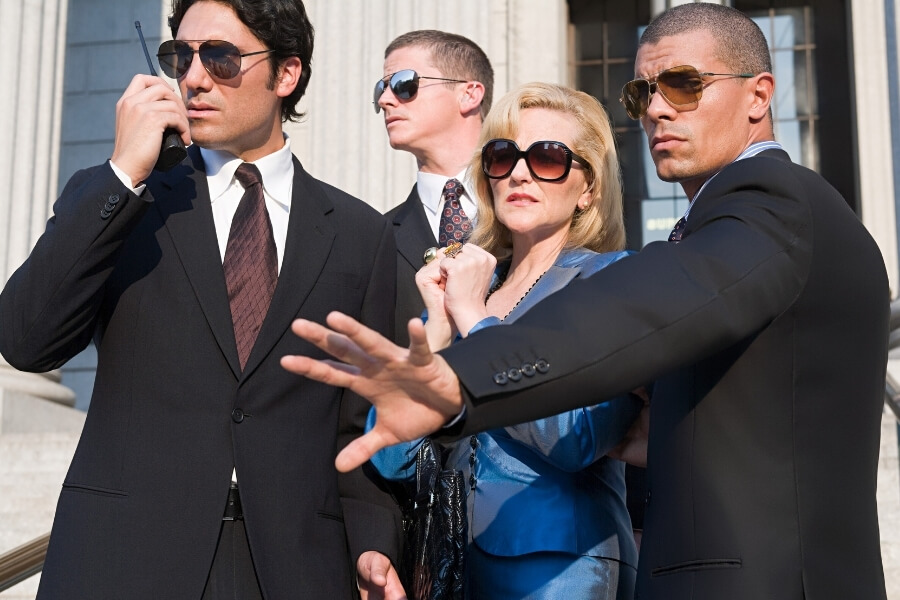
\includegraphics[width=0.4\textwidth]{img/Celebrities-and-entertainers.jpg}
        \caption{Przykład wizualizacji gry}
        \label{fig:real_b_p}
    \end{figure}
\end{frame}

\begin{frame}{Ochroniarze i prezydent}
    Dla grafu $G$ o $n$ wierzchołkach $B\left(G\right) = n-1$.
    W takiej sytuacji przy rozstawianiu ochroniarze już okupują $n-1$ wierzołków. 
    Prezydent ma wtedy dwie opcje, wybrać wierzchołek z ochroniarzem\dots \onslide<3->{lub bez.}
    \begin{figure}
        \begin{columns}[t]
            \column{.5\textwidth}
                \centering
                \onslide<1->{
                    \begin{tikzpicture}
                        \node[cop_vertex] (v1) at (0,1) {1};
                        \node[cop_vertex] (v2) at (1,0) {2};
                        \node[cop_vertex] (v3) at (3,0) {3};
                        \node[cop_vertex] (v4) at (4,1) {4};
                        \node[cop_rob_vertex] (v5) at (3,2) {5};
                        \node[vertex] (v6) at (1,2) {6};
                        
                        \draw[edge] (v1)--(v2);
                        \draw[edge] (v1)--(v3);
                        \draw[edge] (v1)--(v4);
                        \draw[edge] (v1)--(v5);
                        \draw[edge] (v1)--(v6);
                        \draw[edge] (v2)--(v3);
                        \draw[edge] (v2)--(v4);
                        \draw[edge] (v2)--(v5);
                        \draw[edge] (v2)--(v6);
                        \draw[edge] (v3)--(v4);
                        \draw[edge] (v3)--(v5);
                        \draw[edge] (v3)--(v6);
                        \draw[edge] (v4)--(v5);
                        \draw[edge] (v4)--(v6);
                        \draw[edge] (v5)--(v6);
                    \end{tikzpicture}
                    \caption{Prezydent zaczynająca na wierzchołku ochroniarza (kolor zielony)}
                }
                \column{.5\textwidth}
                \centering
                \onslide<2->{
                    \begin{tikzpicture}
                        \node[cop_vertex] (v1) at (0,1) {1};
                        \node[cop_vertex] (v2) at (1,0) {2};
                        \node[cop_vertex] (v3) at (3,0) {3};
                        \node[cop_vertex] (v4) at (4,1) {4};
                        \node[rob_vertex] (v5) at (3,2) {5};
                        \node[cop_vertex] (v6) at (1,2) {6};
                        
                        \draw[edge] (v1)--(v2);
                        \draw[edge] (v1)--(v3);
                        \draw[edge] (v1)--(v4);
                        \draw[edge] (v1)--(v5);
                        \draw[edge] (v1)--(v6);
                        \draw[edge] (v2)--(v3);
                        \draw[edge] (v2)--(v4);
                        \draw[edge] (v2)--(v5);
                        \draw[edge] (v2)--(v6);
                        \draw[edge] (v3)--(v4);
                        \draw[edge] (v3)--(v5);
                        \draw[edge] (v3)--(v6);
                        \draw[edge] (v4)--(v5);
                        \draw[edge] (v4)--(v6);
                        \draw[edge] (v5)--(v6);
                    \end{tikzpicture}
                    \caption{Po pierwszym ruchu ochroniarzy}
                }
        \end{columns}
    \end{figure}  
    \onslide<4>{Jak widać po powyższym przykładzie, grę można podzielić na 2 fazy, okrążenia i utrzymania okrążenia}
\end{frame}

\begin{frame}{Ochroniarze i prezydent}
    \begin{lemma}
        Dla każdego grafu $G$, $B\left(G\right)\ge \Delta\left(G\right)$.
    \end{lemma}
    \pause
    \begin{proof}
        Jeżeli prezydent stoi na wierzchołku o największym stopniu,
        ochroniarze nie mogą wygrać nie okrążając prezydent na tym wierzchołku.
    \end{proof}
    \begin{examples}<3>
        \begin{figure}
            \begin{columns}[t]
                \column{.2\textwidth}
                    \centering
                        \begin{tikzpicture}
                            \node[cop_vertex] (v1) at (0,0) {1};
                            \node[rob_vertex] (v2) at (0,1) {2};
                            \node[vertex] (v3) at (0,2) {3};

                            \draw[edge] (v1)--(v2);
                            \draw[edge] (v2)--(v3);
                        \end{tikzpicture}
                \column{.5\textwidth}
                    \centering
                        \begin{tikzpicture}
                            \node[cop_vertex] (v1) at (0,1) {1};
                            \node[cop_vertex] (v2) at (1,0) {2};
                            \node[cop_vertex] (v3) at (3,0) {3};
                            \node[cop_vertex] (v4) at (4,1) {4};
                            \node[cop_vertex] (v5) at (3,2) {5};
                            \node[cop_vertex] (v6) at (1,2) {6};
                            \node[rob_vertex] (v7) at (2,1) {7};
                            \node[vertex] (v8) at (2,2) {8};
                            
                            \draw[edge] (v1)--(v7);
                            \draw[edge] (v2)--(v7);
                            \draw[edge] (v3)--(v7);
                            \draw[edge] (v4)--(v7);
                            \draw[edge] (v5)--(v7);
                            \draw[edge] (v6)--(v7);
                            \draw[edge] (v1)--(v2);
                            \draw[edge] (v2)--(v3);
                            \draw[edge] (v3)--(v4);
                            \draw[edge] (v4)--(v5);
                            \draw[edge] (v5)--(v8);
                            \draw[edge] (v6)--(v8);
                            \draw[edge] (v6)--(v1);
                        \end{tikzpicture}
            \end{columns}
        \end{figure}
    \end{examples}
\end{frame}

\begin{frame}{Ochroniarze i prezydent}
    \begin{lemma}
        Dla każdego grafu $G$, $B\left(G\right)\ge \Delta\left(G\right)$.
        \label{lem_B_ge_Delta}
    \end{lemma}
    \begin{examples}
        \begin{figure}
            \begin{columns}[t]
                \column{.5\textwidth}
                    \centering
                    \begin{tikzpicture}
                        \node[cop_vertex] (v1) at (0,1) {1};
                        \node[cop_vertex] (v2) at (1,0) {2};
                        \node[cop_vertex] (v3) at (3,0) {3};
                        \node[cop_vertex] (v4) at (4,1) {4};
                        \node[cop_vertex] (v5) at (3,2) {5};
                        \node[cop_vertex] (v6) at (1,2) {6};
                        \node[rob_vertex] (v7) at (2,1) {7};
                        \node[vertex] (v8) at (5,2) {8};
                        \node[vertex] (v9) at (5,0) {9};
                        
                        \draw[edge] (v1)--(v7);
                        \draw[edge] (v2)--(v7);
                        \draw[edge] (v3)--(v7);
                        \draw[edge] (v4)--(v7);
                        \draw[edge] (v5)--(v7);
                        \draw[edge] (v6)--(v7);
                        \draw[edge] (v1)--(v2);
                        \draw[edge] (v2)--(v3);
                        \draw[edge] (v3)--(v4);
                        \draw[edge] (v4)--(v5);
                        \draw[edge] (v5)--(v6);
                        \draw[edge] (v6)--(v1);
                        \draw[edge] (v4)--(v8);
                        \draw[edge] (v4)--(v9);
                        \draw[edge] (v8)--(v9);
                    \end{tikzpicture}
                \column{.5\textwidth}
                    \centering
                    \begin{tikzpicture}
                        \node[vertex] (v1) at (0,1) {1};
                        \node[cop_vertex] (v2) at (1,0) {2};
                        \node[cop_vertex] (v3) at (3,0) {3};
                        \node[cop_rob_vertex] (v4) at (4,1) {4};
                        \node[cop_vertex] (v5) at (3,2) {5};
                        \node[cop_vertex] (v6) at (1,2) {6};
                        \node[cop_vertex] (v7) at (2,1) {7};
                        \node[cop_vertex] (v8) at (5,2) {8};
                        \node[vertex] (v9) at (5,0) {9};
                        
                        \draw[edge] (v1)--(v7);
                        \draw[edge] (v2)--(v7);
                        \draw[edge] (v3)--(v7);
                        \draw[edge] (v4)--(v7);
                        \draw[edge] (v5)--(v7);
                        \draw[edge] (v6)--(v7);
                        \draw[edge] (v1)--(v2);
                        \draw[edge] (v2)--(v3);
                        \draw[edge] (v3)--(v4);
                        \draw[edge] (v4)--(v5);
                        \draw[edge] (v5)--(v6);
                        \draw[edge] (v6)--(v1);
                        \draw[edge] (v4)--(v8);
                        \draw[edge] (v4)--(v9);
                        \draw[edge] (v8)--(v9);
                    \end{tikzpicture}
            \end{columns}
        \end{figure}
    \end{examples}
\end{frame}

\begin{frame}{Ochroniarze i prezydent}
    \begin{theorem}
        Dla każdego grafu $G$ na n wierzchołkach, 
        $B\left(G\right) = n-1$ wtedy i tylko wtedy, gdy $\Delta\left(G\right) = n-1$. 
    \end{theorem}
    \begin{examples}
        \begin{figure}
            \begin{columns}[t]
                \column{.5\textwidth}
                    \centering
                    \begin{tikzpicture}
                        \node[vertex] (v1) at (0,1) {1};
                        \node[vertex] (v2) at (1,0) {2};
                        \node[vertex] (v3) at (2,0) {3};
                        \node[vertex] (v4) at (3,0) {4};
                        \node[vertex] (v5) at (4,1) {5};
                        \node[vertex] (v6) at (3,2) {6};
                        \node[vertex] (v7) at (2,2) {7};
                        \node[vertex] (v8) at (1,2) {8};
                        \node[vertex] (v9) at (2,1) {9};
                        
                        \draw[edge] (v1)--(v9);
                        \draw[edge] (v2)--(v9);
                        \draw[edge] (v3)--(v9);
                        \draw[edge] (v4)--(v9);
                        \draw[edge] (v5)--(v9);
                        \draw[edge] (v6)--(v9);
                        \draw[edge] (v7)--(v9);
                        \draw[edge] (v8)--(v9);
                        \draw[edge] (v1)--(v2);
                        \draw[edge] (v2)--(v3);
                        \draw[edge] (v3)--(v4);
                        \draw[edge] (v5)--(v6);
                        \draw[edge] (v6)--(v7);
                        \draw[edge] (v7)--(v8);
                    \end{tikzpicture}
                \column{.5\textwidth}
                    \centering
                    \begin{tikzpicture}
                        \node[vertex] (v1) at (0,1) {1};
                        \node[vertex] (v2) at (1,0) {2};
                        \node[vertex] (v3) at (3,0) {3};
                        \node[vertex] (v4) at (4,1) {4};
                        \node[vertex] (v5) at (3,2) {5};
                        \node[vertex] (v6) at (1,2) {6};
                        
                        \draw[edge] (v1)--(v2);
                        \draw[edge] (v1)--(v3);
                        \draw[edge] (v1)--(v4);
                        \draw[edge] (v1)--(v5);
                        \draw[edge] (v1)--(v6);
                        \draw[edge] (v2)--(v3);
                        \draw[edge] (v2)--(v4);
                        \draw[edge] (v2)--(v5);
                        \draw[edge] (v2)--(v6);
                        \draw[edge] (v3)--(v4);
                        \draw[edge] (v3)--(v5);
                        \draw[edge] (v3)--(v6);
                        \draw[edge] (v4)--(v5);
                        \draw[edge] (v4)--(v6);
                        \draw[edge] (v5)--(v6);
                    \end{tikzpicture}
            \end{columns}
        \end{figure}
    \end{examples}
\end{frame}

\begin{frame}{Ochroniarze i prezydent}
    \begin{proof}
        \renewcommand{\qedsymbol}{}
        Jeżeli $\Delta\left(G\right)=n-1$ to z lematu $B\left(G\right)\ge \Delta\left(G\right)$ oraz $B\left(G\right) = n-1$, 
        to $B\left(G\right)=n-1$.
        \pause

        Załóżmy że $\Delta\left(G\right) < n-1$.\\
        \pause
        Dla $n\le3$ $G$ jest izomorficzne do $E_n$, $P_2$, $P_3$ albo $C_3$. $B\left(E_n\right) = 0$, gdyż wierzchołki nie są połączone.
        Można łatwo zauważyć, że $B\left(P_2\right) = 1$, $B\left(P_3\right) = B\left(C_3\right) = 2$. 
        \pause
        \begin{examples}
            \begin{figure}
                \begin{columns}[t]
                    \column{.2\textwidth}
                        \centering
                        \begin{tikzpicture}
                            \node[vertex] (v1) at (0,0) {1};
                            \node[vertex] (v2) at (1,1) {2};
                            \node[rob_vertex] (v3) at (0, 1) {3};
                        \end{tikzpicture}
                        \caption{$E_n$}
                    \column{.2\textwidth}
                        \centering
                        \begin{tikzpicture}
                            \node[cop_vertex] (v1) at (0,0) {1};
                            \node[rob_vertex] (v2) at (1,1) {2};
                                
                            \draw[edge] (v1)--(v2);
                        \end{tikzpicture}
                        \caption{$P_2$}
                    \column{.2\textwidth}
                        \centering
                        \begin{tikzpicture}
                            \node[cop_vertex] (v1) at (0,0) {1};
                            \node[rob_vertex] (v2) at (1,0) {2};
                            \node[cop_vertex] (v3) at (1,1) {2};
                                
                            \draw[edge] (v1)--(v2);
                            \draw[edge] (v2)--(v3);
                        \end{tikzpicture}
                    \caption{$P_3$}
                    \column{.2\textwidth}
                        \centering
                        \begin{tikzpicture}
                            \node[cop_vertex] (v1) at (0,0) {1};
                            \node[rob_vertex] (v2) at (1,0) {2};
                            \node[cop_vertex] (v3) at (1,1) {2};
                                
                            \draw[edge] (v1)--(v2);
                            \draw[edge] (v2)--(v3);
                            \draw[edge] (v1)--(v3);
                        \end{tikzpicture}
                        \caption{$C_2$}
                \end{columns}
            \end{figure}
        \end{examples}
    \end{proof}
\end{frame}

\begin{frame}{Ochroniarze i prezydent}

\end{frame}

\setbeamercovered{transparent}
\begin{frame}[allowframebreaks]{Bibliografia}
    \bibliographystyle{plain}
    \bibliography{bibliography.bib}
\end{frame}

%%% PG LAST PAGE %%%
\pglastframe


%%% DOCUMENT ENDS HERE. Good bye! :) %%%

\end{document}
